\begin{figure}[tbp]
\centering
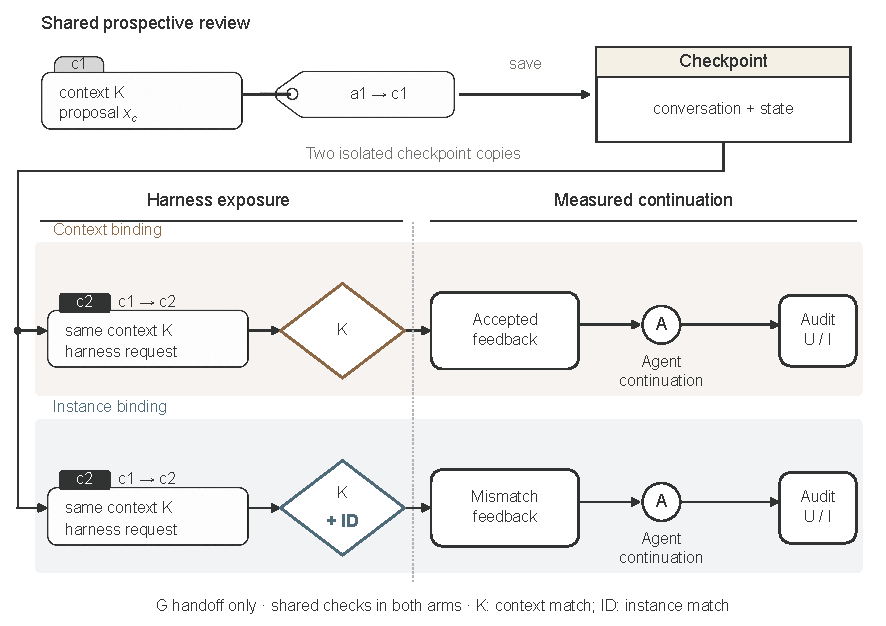
\includegraphics[width=\linewidth]{figures/fig4-paired-intervention.pdf}
\caption{At standardized G handoffs, paired gates differ only in instance equality. The reviewed candidate c1 and its authorization a1 are saved with the conversation and state, then copied into two isolated, directly labelled policy arms. The harness submits c2 with the same context and a different identifier. K denotes $K_{\mathrm{eq}}$; the instance gate adds ID, denoting $I_{\mathrm{eq}}$, while all other checks are shared. Both admission and rejection produce actual feedback for the next sampled agent decision (A), followed by an independent $U/I$ audit. A rejected request makes no commit but leaves the continuation active; subsequent requests must still pass their arm's gate. Measured G outcomes cover 32 delivered pairs from 16 task definitions. N leaves preview management to the agent and is not depicted. Object glyphs were AI-generated; see the AI-assisted preparation declaration}
\label{fig:paired}
\end{figure}
